\begin{figure*}[hbt!]
    \centering
    \subfloat[AlexNet Feature]{
        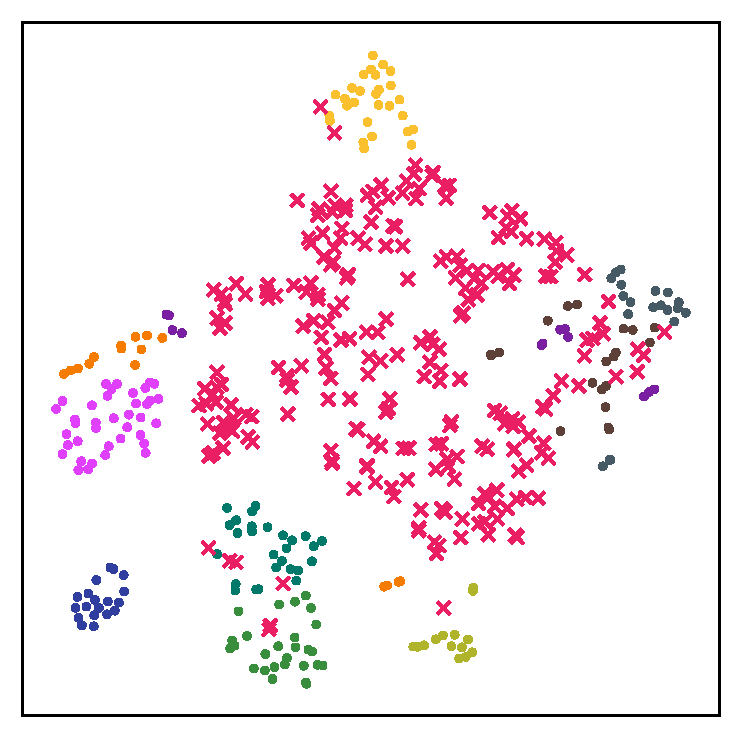
\includegraphics[width=0.235\textwidth]{contents/figures/pdf/tsne/Source.pdf} 
        \label{figure: tSNE source}
    } 
    % \hfil
    \subfloat[GRL Feature]{
        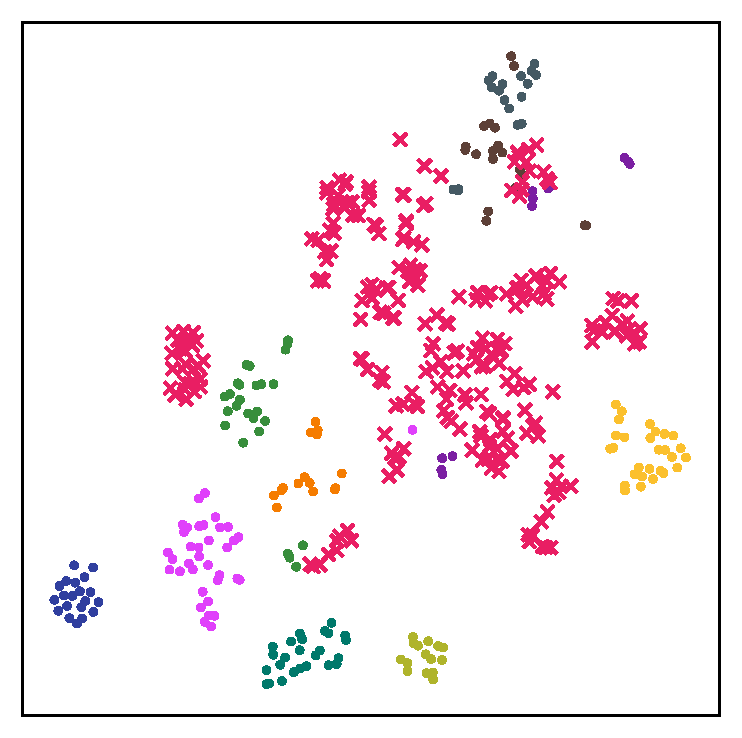
\includegraphics[width=0.235\textwidth]{contents/figures/pdf/tsne/DANN.pdf} 
        \label{figure: tSNE RGL}
    }
    % \hfil
    \subfloat[OSBP Feature]{
        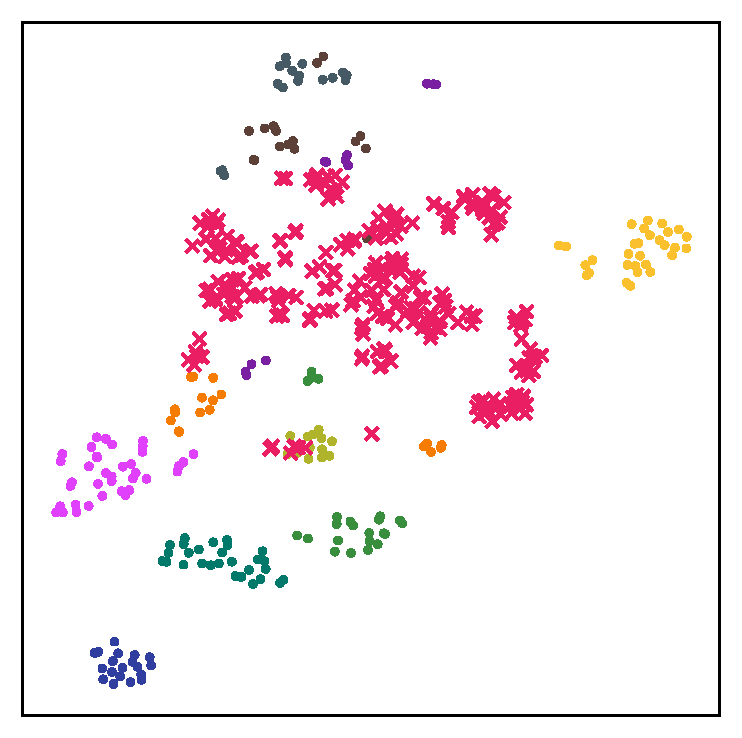
\includegraphics[width=0.235\textwidth]{contents/figures/pdf/tsne/OSBP.pdf} 
        \label{figure: tSNE OSBP}
    }
    % \hfil
    \subfloat[ThDAN Feature]{
        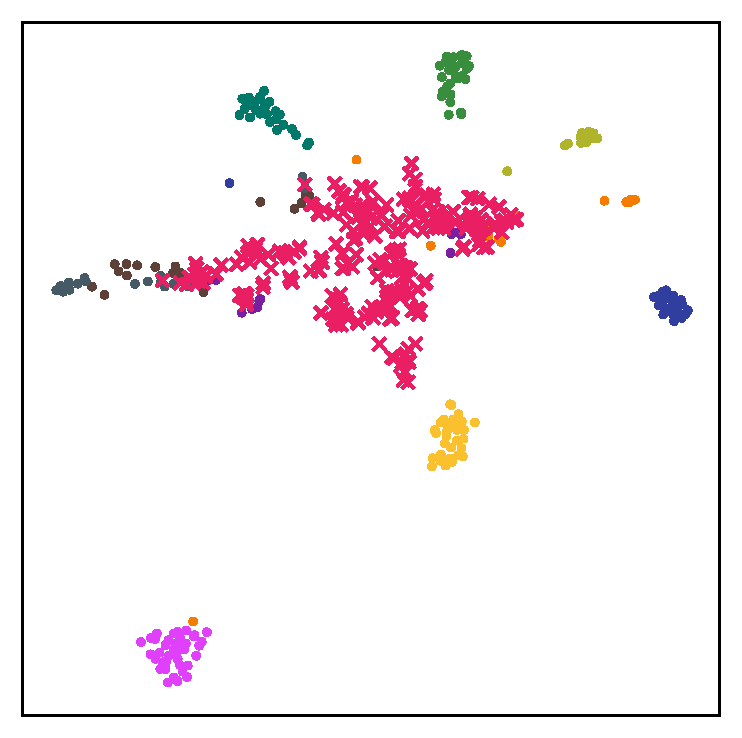
\includegraphics[width=0.235\textwidth]{contents/figures/pdf/tsne/ThDAN.pdf} 
        \label{figure: tSNE ThDAN}
    }
    \caption{
        The t-SNE visualization of obtained target features. The red cross '\unknowncolor{\textbf{$\scriptstyle\times$}}' indicate the unknown target examples, and porint of different colors indicate different known class. 
        (\textbf{a}): Feature obtained by AlexNet trained on the source domain. 
        (\textbf{b}): Features obtained by a model trained with Gradient Reversal Layer. 
        (\textbf{c}): Features obtained by OSBP. 
        (\textbf{d}): Features obtained by our model.
    } \label{figure: tSNE}
\end{figure*}

